% !TeX spellcheck = de_DE


\newglossaryentry{dataset}
{name={Daten},
	description={Ein Datensatz\index{Daten} (Daten) besteht aus einem oder mehreren Datenpunkten 
		und ist eine zentrale Komponente der meisten KI Anwendungen. Diese Anwendungen 
		verwenden Datensätze zum Trainieren und Validieren von KI-Modellen. Verschiedene 
		mathematische Modelle und formale Sprachen wurden entwickelt um Datensätze 
		zu beschreiben und zu analysieren \cite{silberschatz2019database,abiteboul1995foundations,hoberman2009data,ramakrishnan2002database}.  
		Eines der am weitesten verbreiteten Datenmodelle ist das relationale Modell, das 
		Daten in Tabellen (oder Beziehungen) organisiert \cite{silberschatz2019database}.
		Eine Tabelle besteht aus Zeilen und Spalten:
		\begin{itemize} 
			\item Jede Zeile der Tabelle repräsentiert einen einzelnen Datenpunkt.
			\item Jede Spalte der Tabelle entspricht einem bestimmten Attribut (oder Merkmal) der 
			Datenpunkte. 
		\end{itemize}
		Tabelle \ref{tab:temperature} zeigt beispielsweise einen Datensatz mit Wetterbeobachtungen.
		\begin{table}[ht]
			\centering
			\begin{tabular}{|l|c|c|c|c|c|}
				\hline
				\textbf{FMI Station} & \textbf{Year} & \textbf{Month} & \textbf{Day} & \textbf{Time} & \textbf{Temp. [°C]} \\ 
				\hline
				Kustavi Isokari & 2023 & 4 & 1 & 00:00 & -0.2 \\ \hline
				Kustavi Isokari & 2023 & 4 & 2 & 00:00 & -0.1 \\ \hline
				Kustavi Isokari & 2023 & 4 & 3 & 00:00 & -1.0 \\ \hline
				Kustavi Isokari & 2023 & 4 & 4 & 00:00 & -0.4 \\ \hline
				Kustavi Isokari & 2023 & 4 & 5 & 00:00 & 0.9 \\ \hline
			\end{tabular}
			\caption{Beobachtungen der Wetter-Station nahe der finnischen Gemeinde \emph{Kustavi}.}
			\label{tab:temperature}
		\end{table}
		Im relationalen Modell ist die Reihenfolge der Zeilen irrelevant und für 
		jedes Attribut (Spalte) muss ein Wertebereich definiert sein. Diese Wertebereiche 
		entsprechen dem Merkmalsraum der Datenpunkte. Während das relationale Modell
		ein nützliches Instrument für die Beschreibung und Analyse von KI System bietet, ist 
		es unzureichend für die Dokumentation von vertrauenswürdiger KI. Moderne Ansätze wie
		Datenblätter für Datensätze bieten eine umfassendere Dokumentation, einschließlich Details 
		zum Erfassungsprozess des Datensatzes und zur beabsichtigten Verwendung \cite{DatasheetData2021}.},first={dataset},text={dataset}  
}





\newglossaryentry{classification}
{name={Klassifizierung},
	description={Klassifizierung\index{Klassifizierung} bezeichnet ML Anwendungen die darauf abzielen, 
		Datenpunkte in eine von mehreren vorgegebenen Kategorien oder Klassen einzuordnen.
	},first={Klassifizierung},text={Klassifizierung} 
}

\newglossaryentry{optimism_in_face_of_uncertainty}
{name={Optimismus im Angesicht der Unsicherheit},
	description={
		\index{Optimismus im Angesicht der Unsicherheit}
		ML-Methoden verwenden ein Leistungsmaß $\bar{f}(\weights)$ um Modell-Parameter $\weights$ 
		zu lernen. Allerdings haben sie in der Regel keinen direkten Zugriff auf $\bar{f}(\weights)$, 
		sondern nur auf eine Schätzung (oder Annäherung) $f(\weights)$. Zum Beispiel verwenden herkömmliche 
		ML Methoden einen Trainingsfehler als Schätzung für den erwarteten Verlust. 
		Mit einem probabilistischen Modell lässt sich ein Konfidenzintervall $\big[ l^{(\weights)},  u^{(\weights)} \big]$ für jede Wahl von Modellparametern konstruieren. 
		Eine einfache Konstruktion hierfür ist $l^{(\weights)} \defeq f(\weights) - \sigma/2$, $u^{(\weights)} \defeq f(\weights) + \sigma/2$, 
		wobei $\sigma$ ein Maß für die (erwartete) Abweichung von $f(\weights)$ zu $\bar{f}(\weights)$ ist. 
		Es können auch andere Konstruktionen für dieses Intervall verwendet werden, solange sie sicherstellen, 
		dass mit ausreichend hoher Wahrscheinlichkeit $\bar{f}(\weights) \in \big[ l^{(\weights)},  u^{(\weights)} \big]$ gilt. 
		Als Optimist wählen wir $\weights$ gemäß dem günstigsten – aber dennoch plausiblen – Wert 
		$\tilde{f}(\weights) \defeq l^{(\weights)}$ des Leistungsmaßes. Zwei Beispiele für diese Konstruktion 
	    findet man in der strukturellen Risikominimierung \cite[Kap. 11]{ShalevMLBook} sowie bei Methoden für 
	    die sequentielle Entscheidungsfindung 
	    \cite[Abschnitt 2.2]{Bubeck2012}. 
		\begin{figure}[htbp]
			\begin{center}
				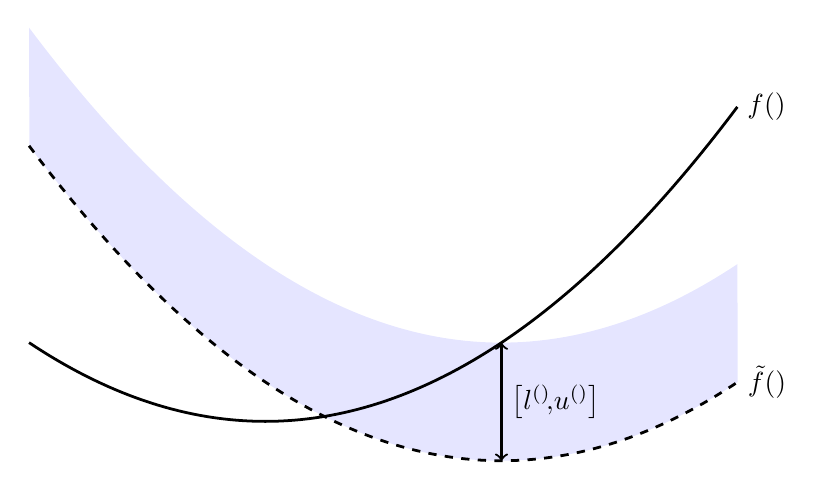
\begin{tikzpicture}[x=3cm, y=1cm]
					% Filled band around the quadratic curve with different boundary curves
					\fill[blue!10] 
					(-1, 5) -- plot[domain=-2:1, samples=100] ({\x+1}, {\x*\x + 1}) -- 
					plot[domain=1:-2, samples=100] ({\x+1}, {\x*\x - 0.5}) -- cycle;
					\node[anchor=west] at (2, 4) {$f(\weights)$};
					\draw[line width=1, domain=-2:1, samples=100,dashed] plot  ({\x+1}, {\x*\x -0.5}) node[right] {$\tilde{f}(\weights)$};
					\draw[line width=1, domain=-1:2, samples=100] plot ({\x}, {\x*\x});
					\draw[<->, thick] (1, -0.5) -- (1, 1) node[midway, right] {$\big[ l^{(\weights)}\!,\!u^{(\weights)} \big]$};
				\end{tikzpicture}
				\caption{Wir verwenden eine Schätzung $f(\weights)$ für das Leistungsmaß $\bar{f}(\weights)$ 
					um ein Konfidenzintervall $\big[ l^{(\weights)},  u^{(\weights)} \big]$ zu konstruieren. Ein Optimist 
					im Angesicht der Unsicherheit wählt Modellparameter $\weights$ gemäß dem günstigsten –
					 aber dennoch plausiblen – Wert $\tilde{f}(\weights) \defeq l^{(\weights)}$.} 
			\end{center}
	\end{figure}},first={Optimismus im Angesicht der Unsicherheit},text={Optimismus im Angesicht der Unsicherheit} 
}
\newglossaryentry{minimum}
{
	name=Minimum,
	description={Bei gegebener Menge reeller Zahlen ist das Minimum \index{Minimum} die kleinste der gegebenen reellen Zahlen.},
	first={Minimum},text={Minimum}
}

\newglossaryentry{maximum}
{name=Maximum,
 description={Bei gegebener Menge reeller Zahlen, ist das Maximum \index{Maximum} die grösste der gegebenen Zahlen.},
 first={Maximum},text={Maximum}
}

\newglossaryentry{discrepancy}
{name=Diskrepanz,
	description={

	Betrachten wir eine \gls{fl}-Anwendung  mit \gls{Netzdaten}, dargestellt durch einen \gls{empgraph}. \gls{fl}-Methoden
	verwenden ein Diskrepanzmaß zum Vergleich von \gls{Hypothese}-Karten aus lokalen Modellen an Knoten $\nodeidx,\nodeidx'$ 
		die durch eine Kante im \gls{empgraph} verbunden sind. }
	first={Diskrepanz},text={Diskrepanz}
}



\newglossaryentry{hfl}
{name={horizontales \gls{fl}},description=


	Horizontales  \gls{fl}\index{horizontales FL} nutzt \gls{lokale datensets} bestehend aus verschiedenen  \gls{Daten punkt}en die durch 
	 die selben \gls{Merkmal}e charakterisiert werden \cite{HFLChapter2020}. Wettervorhersagen zum Beispiel nutzen ein Netwerk aus räumlich 
	 verteilten Wetter(beobachtungs)stationen. Jeder Wetterstation misst dieselben Größen wie die tägiche Temperature, Luftdruck und den Niederschlag. 
	 Verschiedene Wetterstationen messen die Charakteristiken oder \gls{Merkmal}e verschiedener räumlich-zeitlicher Regionen.Jede räumlich-zeitliche
	 Region  steht für einen \gls{Daten punkt} der charakterisiert is durch die selben Merkmale (zum Beipiel die tägliche Temperatur oder den Luftdruck).
	 first={Horizontales \gls{fl}},text={horizontales \gls{fl}}
	}
	
}

\newglossaryentry{dimred}
{name={Dimensionalitätsreduktion},


description={Methoden zur Dimensionalitätsreduktion \index{Dimensionalitätsreduktion} bilden (typischer viele)
rohe \gls{Merkmal}e auf eine (relativ kleine) Menge von neuen \gls{Merkmal}en ab. Diese Methoden können genutzt werden um \gls{Daten punkt}e 
zu visualisieren indem zwei \gls{Merkmal}e erlent werden die als Koordinaten fuer eine Darstellung in einem \gls{Streudiagramm} verwerden werden. }, 
first={Dimensionalitätsreduktion},text={Dimensionalitätsreduktion}

}

	
\newglossaryentry{featlearn}
{name={Merkmalslernen},

description={Betrachten wir eine Anwendung Maschinellen Lernens mit Datenpunkten, die durch \emph{rohe} \gls{Merkmal}e gekennzeichnet sind $\featurevec \in \featurespace$.
Merkmalslernen bezieht sich auf die Aufgabe eine Abbildung $$\featuremapvec: \featurespace \rightarrow \featurespace': \featurevec \mapsto \featurevec',$$ zu erlernen, die die rohen \gls{Merkmal}e $\featurevec \in \featurespace$ 
eines \gls{Daten punkt}s einliest und neue \gls{Merkmal}e  $\featurevec' \in \featurespace'$  in einem neuen  \gls{Merkmalsraum} $\featurespace'$ liefert. 
Verschiedene  Methoden der \gls{Merkmalserfassung} werden durch verschiedene Designentscheidungen für  $\featurespace,\featurespace'$,  einen \gls{Hypothesenraum} $\hypospace$  für potentielle Abbildungen $\featuremapvec$ und ein quantitatives 
Maß für die Nützlichkeit einer spezifischen $\featuremapvec \in \hypospace$ ermittelt.
Zum Beispiel verwendet die  \gls{Hauptkomponentenanalyse} $\featurespace \defeq \mathbb{R}^{\dimlocalmodel}$, $\featurespace' \defeq \mathbb{R}^{\dimlocalmodel'}$ mit $\dimlocalmodel' < \dimlocalmodel$ und 
dem \gls{Hypothesenraum} $$\hypospace\defeq \big\{ \featuremapvec: \mathbb{R}^{\dimlocalmodel}
\!\rightarrow\! \mathbb{R}^{\dimlocalmodel'}\!:\!\featurevec'\!\defeq\!\mF \featurevec \mbox{ with some } \mF \!\in\! \mathbb{R}^{\dimlocalmodel' \times \dimlocalmodel} \big\}.$$
Die \gls{Hauptkomponentenanalyse} misst die Nützlichkeit einer spezifischen Abbildung $\featuremapvec(\featurevec)= \mF \featurevec$ durch den minimalen linearen Rekonstruktionsfehler, der auf einem \gls{Datensatz} auftritt: 
$$ \min_{\mG \in \mathbb{R}^{\dimlocalmodel \times \dimlocalmodel'}} \sum_{\sampleidx=1}^{\samplesize} \normgeneric{\mG \mF \featurevec^{(\sampleidx)} - \featurevec^{(\sampleidx)}}{2}^{2}.$$ }, 
first={Merkmalslernen},text={Merkmalslernen}

\newglossaryentry{Autoencoder}
{name={Autoencoder},
	description={Ein Autoencoder \index{Autoencoder} ist eine ML Methode die gleichzeitig eine Encoder(Kodierer) Karte $\hypothesis(\cdot) \in \hypospace$  und eine decoder (Dekodierer) Karter erlernt $\hypothesis^{*}(\cdot) \in \hypospace^{*}$.
	Es handelt sich um eine Instanz von \gls{erm} unter Verwendung eines \gls{loss}, der aus dem Rekonstruktionsfehler berechnet wird 
		$\featurevec - \hypothesis^{*}\big( \hypothesis \big( \featurevec \big) \big)$.},
	first={Autoencoder},text={Autoencoder}
} 

\newglossaryentry{vfl}
{name={vertikale \gls{fl}},description=
	{Vertikale \gls{fl}\index{vertical FL} uses \gls{localdataset}s that are constituted 
	 by the same \gls{datapoint}s but characterizing them with different \gls{feature}s \cite{VFLChapter}. 
     For example, different healthcare providers might all contain information 
     about the same population of patients. However, different healthcare providers 
     collect different measurements (blood values, electrocardiography, lung X-ray) 
     for the same patients.},
	first={vertical \gls{fl}},text={vertical \gls{fl}}
} 

\newglossaryentry{interpretability}
{name={interpretability},description=
		{Eine Methode Maschinellen Lernens is interpretierbar \index{interpretability} wenn ein spezifischer Nutzer die Vorhersage  gut antizipieren kann. 
		Interpretierbarkeit kann quantifiert werden in dem man die Unsicherheit gegenüber einer Vorhersage betrachtet \cite{JunXML2020}.
		first={Interpretierbarkeit},text={Interpretierbarkeit}		
		An ML method is interpretable\index{interpretability} for a specific user if 
			they can anticipate the \gls{prediction}s delivered by the method well. 
			The notion of interpretability can be made precise using quantitative 
			measures of the uncertainty about the \gls{prediction}s \cite{JunXML2020}.},
		first={interpretability},text={interpretability}
		}

		newglossaryentry{multitask learning}
		{name={Multitasklernen},description=
			{Multitask lernen\index{multitask learning} aims at leveraging relations between 
			 different \gls{learningtask}s. Consider two \gls{learningtask}s obtained from the 
			 same \gls{dataset} of webcam snapshots. The first task is to predict the presence 
			 of a human, while the second is the predict the presence of a car. It might be useful 
			 to use the same \gls{deepnet} structure for both tasks and only allow the weights of 
			 the final output layer to be different.},
			first={multitask learning},text={multitask learning}
		}
		
		\newglossaryentry{learningtask}
		{name={Lernaufgabe},description=
			{Consider\index{learning task} a \gls{dataset} $\dataset$ constituted by several \gls{datapoint}s, each of them 
			 characterized by \gls{feature}s $\featurevec$. For example, the \gls{dataset} $\dataset$ 
			 might be constituted by the images of a particular database. Sometimes it might be useful 
			 to represent a \gls{dataset} $\dataset$, along with the choice of \gls{feature}s, by a \gls{probdist} $p(\featurevec)$. 
			 A learning task associated with $\dataset$ consists of a specific 
			 choice for the \gls{label} of a \gls{datapoint} and the corresponding \gls{labelspace}. 
			 Given a choice for the \gls{lossfunc} and \gls{model}, a learning task gives rise to an 
			 instance of \gls{erm}. Thus, we could define a learning task also via an instance of \gls{erm}, i.e., 
			 via an objective function.  Note that, for the same \gls{dataset}, we obtain different learning tasks by using 
			 different choices for the \gls{feature}s and \gls{label} of a \gls{datapoint}. These learning 
			 tasks are related, as they are based on the same \gls{dataset}, and solving them jointly 
			 (via multitask learning methods) is typically preferable over solving them separately \cite{Caruana:1997wk,JungGaphLassoSPL,CSGraphSelJournal}.},
			first={learning task},text={learning task}
		}
		
		\newglossaryentry{explainability}
		{name={explainability},description=
				{We\index{explainability} define the (subjective) explainability of an ML method 
					as the level of simulatability \cite{Colin:2022aa} of the \gls{prediction}s 
					delivered by an ML system to a human user. Quantitative measures for the 
					(subjective) explainability of a trained \gls{model} can be constructed by 
					comparing its \gls{prediction}s with the \gls{prediction}s provided by a user 
					on a \gls{testset} \cite{Zhang:2024aa,Colin:2022aa}. Alternatively, we can use 
					\gls{probmodel}s for \gls{data} and measure the explainability of a trained ML model 
					via the conditional (differential) entropy of its \gls{prediction}s, given the user \gls{prediction}s \cite{JunXML2020,Chen2018}. 
				},
				first={explainability},text={explainability}
			}
		
		\newglossaryentry{linmodel}{name={linear model},
			description={Consider\index{linear model}  \gls{datapoint}s, each characterized by a numeric \gls{feature} 
				vector $\featurevec \in \mathbb{R}^{\featuredim}$. A linear \gls{model} is 
				a \gls{hypospace} which consists of all linear maps, 
			\begin{equation} 
				\label{equ_def_lin_model_hypspace}
				\linmodel{\nrfeatures} \defeq \left\{ \hypothesis(\featurevec)= \weights^{T} \featurevec: \weights \in \mathbb{R}^{\nrfeatures} \right\}. 
			\end{equation} 
			Note that \eqref{equ_def_lin_model_hypspace} defines an entire family of \gls{hypospace}s, which is 
			parameterized by the number $\nrfeatures$ of \gls{feature}s that are linearly combined to form the 
			\gls{prediction} $\hypothesis(\featurevec)$. The design choice of $\nrfeatures$ is guided by \gls{compasp} 
			(smaller $\nrfeatures$ means less computation), \gls{statasp} (increasing $\nrfeatures$ might 
			reduce \gls{prediction} error) and \gls{interpretability}. A linear \gls{model} using few carefully chosen 
			\gls{feature}s tends to be considered more interpretable \cite{Ribeiro2016,rudin2019stop}.}, 
		   first={linear model},text={linear model}}
			
			
		\newglossaryentry{gradstep}{name={gradient step},description={Given a \gls{differentiable} 
				real-valued function $f(\cdot): \mathbb{R}^{\nrfeatures} \rightarrow \mathbb{R}$ 
				 and a vector $\weights \in \mathbb{R}^{\nrfeatures}$, the \gls{gradient} step\index{gradient step} 
				 updates $\weights$ by adding the scaled negative \gls{gradient} $\nabla f(\weights)$ to obtain 
				 the new vector (see Fig.\ \ref{fig_basic_GD_step_single})
				 \begin{equation}
				 \label{equ_def_gd_basic} 
				\widehat{\weights}  \defeq \weights - \lrate \nabla f(\weights).
				\end{equation} 
				Mathematically, the gradient step is a (typically non-linear) operator $\mathcal{T}^{(f,\lrate)}$ 
				that is parametrized by the function $f$ and the \gls{stepsize} $\lrate$. 
				\begin{figure}[htbp]
					\begin{center}
						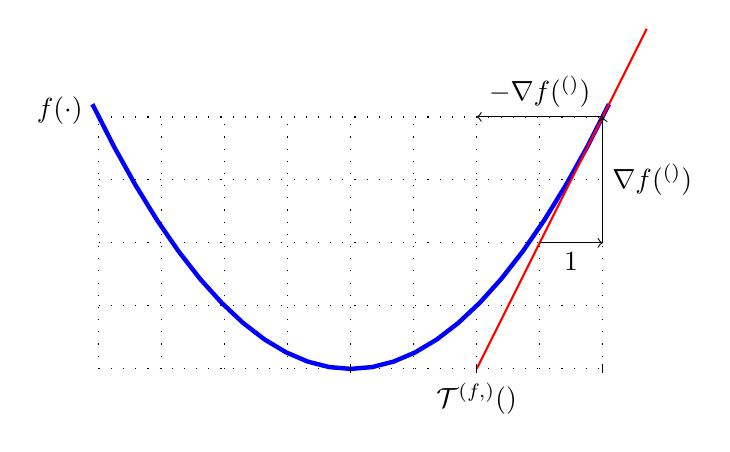
\begin{tikzpicture}[scale=0.8]
							\draw[loosely dotted] (-4,0) grid (4,4);
							\draw[blue, ultra thick, domain=-4.1:4.1] plot (\x,  {(1/4)*\x*\x});
							\draw[red, thick, domain=2:4.7] plot (\x,  {2*\x - 4});
							\draw[<-] (4,4) -- node[right] {$\nabla f(\weights^{(\itercntr)})$} (4,2);
							\draw[->] (4,4) -- node[above] {$-\lrate \nabla f(\weights^{(\itercntr)})$} (2,4);
							\draw[<-] (4,2) -- node[below] {$1$} (3,2) ;
							%\draw[->] (-4.25,0) -- (4.25,0) node[right] {$a$};
							\node[left] at (-4.1, 4.1) {$f(\cdot)$}; 
							\draw[shift={(0,0)}] (0pt,2pt) -- (0pt,-2pt) node[below] {$\overline{\weights}$};
							\draw[shift={(4,0)}] (0pt,2pt) -- (0pt,-2pt) node[below] {$\weights$};
							\draw[shift={(2,0)}] (0pt,2pt) -- (0pt,-2pt) node[below] {$\mathcal{T}^{(f,\lrate)}(\weights)$};
						\end{tikzpicture}
					\end{center}
					\caption{The basic gradient step \eqref{equ_def_gd_basic} maps a given vector $\weights$ 
					to the updated vector $\weights'$. It defines an operator 
					$\mathcal{T}^{(f,\lrate)}(\cdot): \mathbb{R}^{\nrfeatures} \rightarrow \mathbb{R}^{\nrfeatures}:
					 \weights \mapsto \widehat{\weights}$.}
					\label{fig_basic_GD_step_single}
				\end{figure}
				Note that the gradient step \eqref{equ_def_gd_basic} optimizes locally - 
				in a neighbourhood whose size is determined by the \gls{stepsize} $\lrate$ - a linear approximation 
				to the function $f(\cdot)$. A natural generalization of \eqref{equ_def_gd_basic} is to locally 
				optimize the function itself - instead of its linear approximation - 
				\begin{align} 
				\label{equ_approx_gd_step}
				\widehat{\weights} = \argmin_{\weights' \in \mathbb{R}^{\dimlocalmodel}} f(\weights')\!+\!(1/\lrate)\normgeneric{\weights-\weights'}{2}^2. 
				\end{align}
				We intentionally use the same symbol $\lrate$ for the parameter in \eqref{equ_approx_gd_step} 
				as we used for the step size in \eqref{equ_def_gd_basic}. The larger we choose $\lrate$ in 
				\eqref{equ_approx_gd_step}, the more progress the update will make towards reducing the 
				function value $f(\widehat{\weights})$. Note that, much like the gradient step \eqref{equ_def_gd_basic}, 
				also the update \eqref{equ_approx_gd_step} defines a (typically non-linear) operator 
				that is parametrized by the function $f(\cdot)$ and the parameter $\lrate$. For a \gls{convex} function 
				$f(\cdot)$, this operator is known as the \gls{proxop} of $f(\cdot)$ \cite{ProximalMethods}. 
				},first={gradient step},text={gradient step}}
